%\subsection{Background}

\begin{figure}[t!]
  \begin{center}
    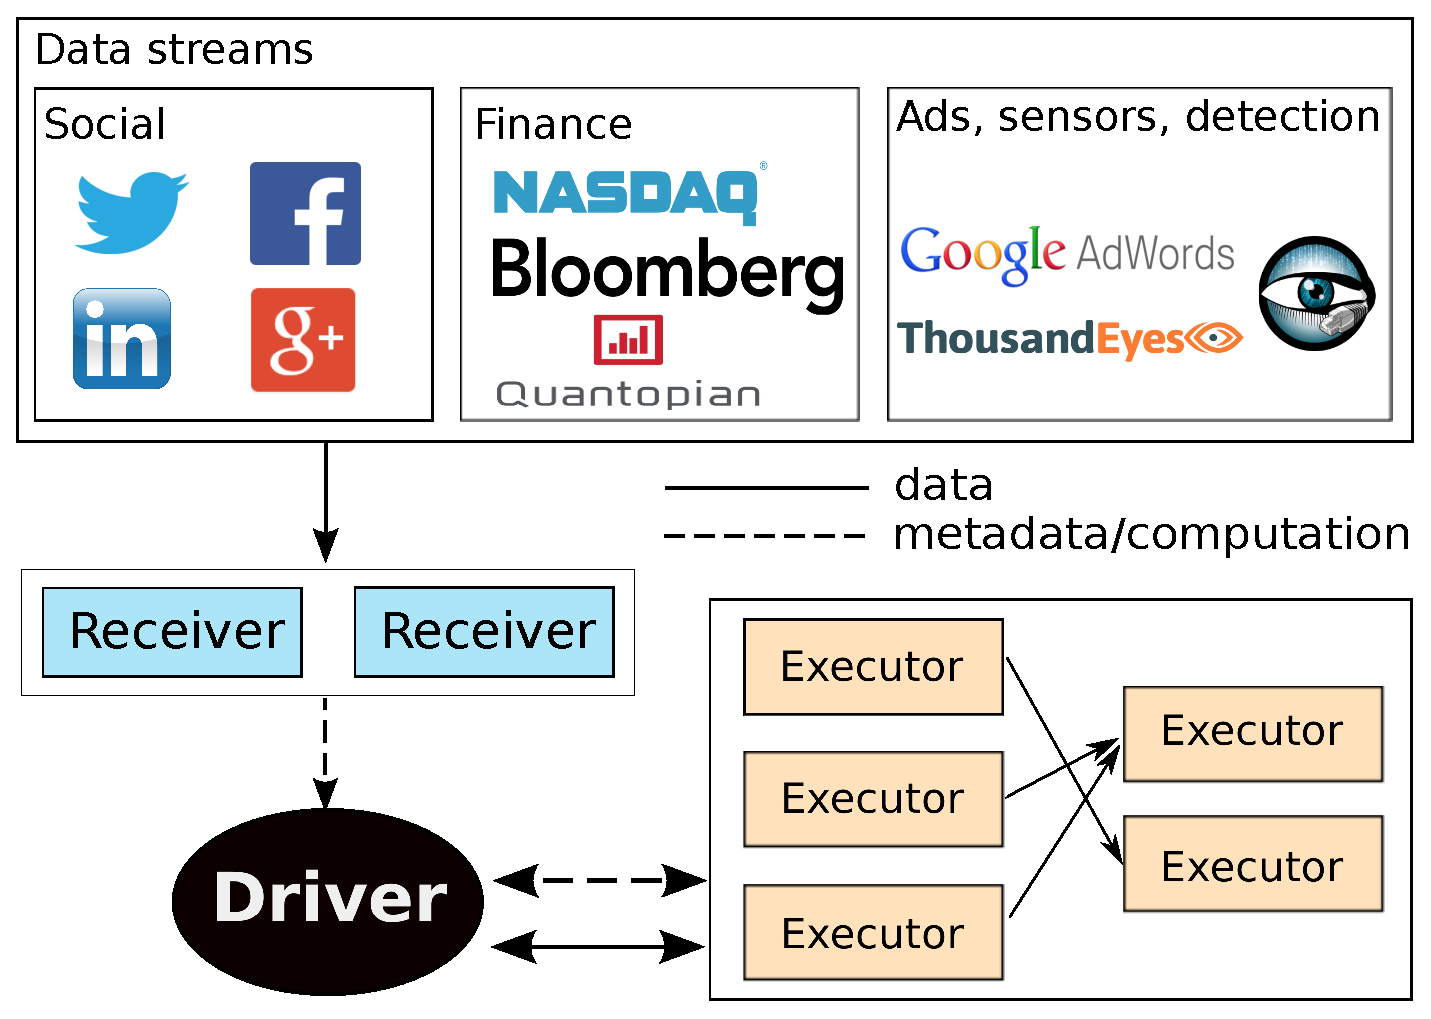
\includegraphics[scale=0.30]{images_graphs/spark_architecture_v4.eps}
  \end{center}
  \caption{Diagram of a Spark Streaming work flow. A Receiver and an Executor may execute in the same node.}
  \label{fig:SparkStreaming_architecture}
\end{figure}

In order to understand the rest of the paper we provide a short description of the architecture of Spark Streaming.

The execution of a Spark Streaming job works as depicted in Figure~\ref{fig:SparkStreaming_architecture}. 
First, data is generated at a source (e.g., tweets from Twitter). As the data is generated it is pushed to Spark Streaming, where it is received by a Receiver. 
The Receiver is responsible for receiving stream data and stash it in memory. Periodically, every <block interval> milliseconds, the Receiver takes the data stashed in memory and generates a block with that data. 
Once a block is generated, the Receiver informs a Spark Streaming's central component called Driver about this block. The Driver is responsible for holding metadata about the records received. 
Periodically, every <batch interval> milliseconds, the Driver takes the blocks that have been communicated by the receivers and that have not been processed yet and generates a batch job. 
Once this batch job is generated it is appended to a queue of jobs to be scheduled. 
The scheduler continuously polls this queue and schedules the jobs in the machines available in the cluster
Jobs are run in stateless isolated environments called Executors. Executors are usually deployed in the same nodes as Receivers.  \joao{is it always like this?}.

Internally, Spark Streaming makes extensive use of Actors -- a design pattern that decouples the invocation of methods from their execution. This means that 
